%%====================================================================
\section{Illustrative Examples}
\label{sec:examples}

\subsection{Research Workflow}

\DIFdelbegin
\DIFdel{ResearchShop supports a compact literature-curation loop: users provide a PubMed query, author search, or PMID list; select papers; define schema columns such as \emph{Key Finding}, \emph{Disease Association}, \emph{Statistical Evidence}, and \emph{Conclusion}; and receive spreadsheet-ready gene--paper rows with provenance and validation metadata. For each selected open-access paper, the pipeline parses text, tables, captions, figures, and supplementary metadata where available; combines PubTator, HGNC scanning, and LLM candidate discovery; fills the requested schema only for grounded candidates; and exports citation status, NCBI identifiers, candidate source, association grouping, confidence label, and paper metadata. The same backend can be run through the desktop interface or from the command line for scripted analyses.}
\DIFdelend

\DIFaddbegin
\DIFadd{Users search PubMed, select open-access papers, and define the fields to extract for each gene or variant. ResearchShop then returns a spreadsheet with the requested fields, source citations, normalized identifiers, and validation metadata. The desktop interface and command-line mode use the same pipeline.}
\DIFaddend

\DIFdelbegin
\DIFdel{Figure~\ref{fig:app_workflow_screens} shows the protocol, query/schema, and results views. Table~\ref{tab:demo_output_trace} uses a local demonstration result file to illustrate the visible data model; it is not an accuracy benchmark.}
\DIFdelend

\DIFdelbegin
\DIFdel{For the example in Figure~\ref{fig:app_workflow_screens}, we searched for \texttt{KRAS AND Poland AND lung cancer} and selected a 2026 Polish cohort study of pulmonary large-cell neuroendocrine carcinoma (PMID 41977128)~\cite{szpechcinski2026lcnec}. The run fetched the full text from PMC, extracted two tables, and produced 42 output rows representing 21 genes in 85.6~s. Two additional candidate rows were rejected because their supplied citations could not be matched to the article. Table~\ref{tab:demo_output_trace} shows three retained rows; this example demonstrates the workflow, not extraction accuracy.}
\DIFdelend

\DIFaddbegin
\DIFadd{For the example in Figure~\ref{fig:app_workflow_screens}, the query was \texttt{(KRAS AND Poland AND lung cancer) AND 2025:2026[dp]}. Table~\ref{tab:demo_output_trace} reports the complete recorded run. The History view's \emph{Genes found} value sums unique genes within each paper, whereas the Results view deduplicates gene labels across the final output. Figure~\ref{fig:app_workflow_screens} also shows an exported \textit{KRAS} G12C row with separate fields and source citations. This example demonstrates output structure and traceability, not extraction accuracy.}
\DIFadd{The recorded duration is retained as run provenance only. The model and complete runtime configuration were not preserved with the supplied workbook, so this value is not compared with the controlled WSL experiment in Section~\ref{sec:impact}.}
\DIFaddend

\subsection{Audit Artifacts}

\DIFdelbegin
\DIFdel{Each run writes the final CSV plus metadata CSV, XLSX, JSON, candidate-audit, drop-debug, and optional trace files. These artifacts record candidate origin, gate outcomes, citation-grounding status, confidence score, fallback paths, and dropped-row reasons. A reviewer can therefore see why a gene appeared, why another was excluded, and whether a supporting sentence was recovered from the paper rather than generated by the LLM.}
\DIFdelend
\LucasNote{To zdanie brzmi jak rasowy LLM}

\DIFdelbegin
\DIFdel{The metadata records which component proposed each row, which validation gates passed or failed, which citation matched article text, and why any row was excluded. During review, an exported row can be traced from the spreadsheet value back to its proposing source, matched citation span, normalized gene identifier, confidence label, and final gate decision without rerunning the LLM.}
\DIFdelend

\DIFaddbegin
\DIFadd{Each run includes the final tables and companion audit files. For every candidate, these files record its source, normalization, validation result, matched citation, and any exclusion reason. Reviewers can therefore check an accepted row against the article text without repeating the LLM call.}
\DIFaddend

\subsection{Figure and Table Handling}

Many genomics papers encode primary findings in figures, tables, and supplementary files rather than in prose. ResearchShop parses PMC and Europe PMC JATS XML, extracts structured table text, collects figure captions and image URL candidates, and passes table/caption context into evidence validation. When figure analysis is enabled and images are downloadable, a multimodal Gemini model is used for analysis.

%can inspect figures as an optional signal; when images are unavailable, the pipeline degrades to caption and text evidence rather than failing the run.

\DIFdelbegin
\DIFdel{The parser path uses ResearchShop-owned fetchers for PubMed, PMC, Europe PMC, and citation services. A small adapter uses \texttt{pubmed\_parser} for selected JATS parsing tasks such as body paragraphs and figure metadata, while ResearchShop keeps its own open-access gates, URL probing, CDN fallback, table extraction, supplementary file handling, PubTator integration, and output schema.}
\DIFdelend
\DIFaddbegin
\DIFadd{ResearchShop owns the fetchers for PubMed, PMC, Europe PMC, and citation services, as well as the open-access gates, URL probing, CDN fallback, table extraction, supplementary file handling, PubTator integration, and output schema. A small adapter uses \texttt{pubmed\_parser} only for selected JATS parsing tasks such as body paragraphs and figure metadata.}
\DIFaddend

\begin{figure*}[t]
\vspace{-0.6em}
\centering
\begingroup
\scriptsize
\captionsetup{hypcap=false}

\DIFdelbegin
\DIFdel{Previous illustrative table and synthetic demonstration rows:}
\par\smallskip
\setlength{\tabcolsep}{3pt}
\renewcommand{\arraystretch}{0.92}
\begin{tabularx}{\textwidth}{@{}>{\raggedright\arraybackslash}p{1.55cm} >{\raggedright\arraybackslash}p{2.15cm} >{\raggedright\arraybackslash}X >{\raggedright\arraybackslash}p{2.75cm}@{}}
\toprule
\DIFdel{\textbf{Output row}} & \DIFdel{\textbf{Candidate source}} & \DIFdel{\textbf{Displayed evidence trail}} & \DIFdel{\textbf{Audit interpretation}} \\
\midrule
\DIFdel{\textit{IFNG}} & \DIFdel{LLM text; deterministic lexicon} & \DIFdel{Gene-normalized immune-response finding with citation status, confidence label, local HGNC validation, and matched source text.} & \DIFdel{Inspect source sentence before reuse.} \\
\DIFdel{\textit{HLA-C} / HLA-C*04} & \DIFdel{LLM text} & \DIFdel{Allele-like input remains in the variant field while the gene label normalizes to an HGNC-compatible symbol.} & \DIFdel{Triage lead; HLA nomenclature requires expert interpretation.} \\
\DIFdel{\textit{CXCL10}} & \DIFdel{PubTator} & \DIFdel{Sparse evidence is retained with a conservative confidence label and needs-review citation status.} & \DIFdel{Visible as a paper index, not a final assertion.} \\
\bottomrule
\end{tabularx}
\DIFdel{Illustrative output and audit trail from a local demonstration result file.}
\DIFdelend

\vspace{0.8em}
\DIFadd{Current example generated from the documented KRAS query:}
\par\smallskip
\setlength{\tabcolsep}{3pt}
\renewcommand{\arraystretch}{0.92}
\begin{tabularx}{\textwidth}{@{}>{\raggedright\arraybackslash}p{4.0cm} >{\raggedright\arraybackslash}p{3.0cm} >{\raggedright\arraybackslash}X@{}}
\toprule
\DIFadd{\textbf{Run measure}} & \DIFadd{\textbf{Recorded value}} & \DIFadd{\textbf{Counting basis}} \\
\midrule
\DIFadd{Duration; API calls} & \DIFadd{141~min 6~s; 31} & \DIFadd{Values recorded in History for the completed run.} \\
\DIFadd{Papers analysed; papers in Results} & \DIFadd{22; 17} & \DIFadd{All analysed papers; papers contributing at least one final row.} \\
\DIFadd{Genes found; globally unique genes} & \DIFadd{185; 107} & \DIFadd{Per-paper unique counts summed; gene labels deduplicated across Results.} \\
\DIFadd{Candidate records; final rows} & \DIFadd{248; 216} & \DIFadd{Candidate Audit records; rows displayed in Results.} \\
\DIFadd{Confidence breakdown} &
\DIFdel{57 corroborated; 85 medium; 2 low; 72 review}
\DIFadd{57 CORROBORATED; 85 SUPPORTED; 2 LIMITED EVIDENCE; 72 NEEDS REVIEW} &
\DIFadd{Final rows mapped to the current review-cue terminology.} \\
\DIFadd{Citation coverage} & \DIFadd{98\%} & \DIFadd{Coverage reported in the Results view.} \\
\bottomrule
\end{tabularx}
\captionof{table}{Recorded summary of the complete KRAS query run supplied for the application example.}
\label{tab:demo_output_trace}

\endgroup
\vspace{-0.6em}
\end{figure*}

\begin{figure*}[t]
\vspace{-0.6em}
\centering
\begingroup
\scriptsize
\captionsetup{hypcap=false}

\vspace{0.8em}
\DIFdelbegin
\DIFdel{Previous three-screen workflow illustration removed.}
\DIFdelend

\vspace{0.8em}
\DIFadd{Current application example:}
\par\smallskip
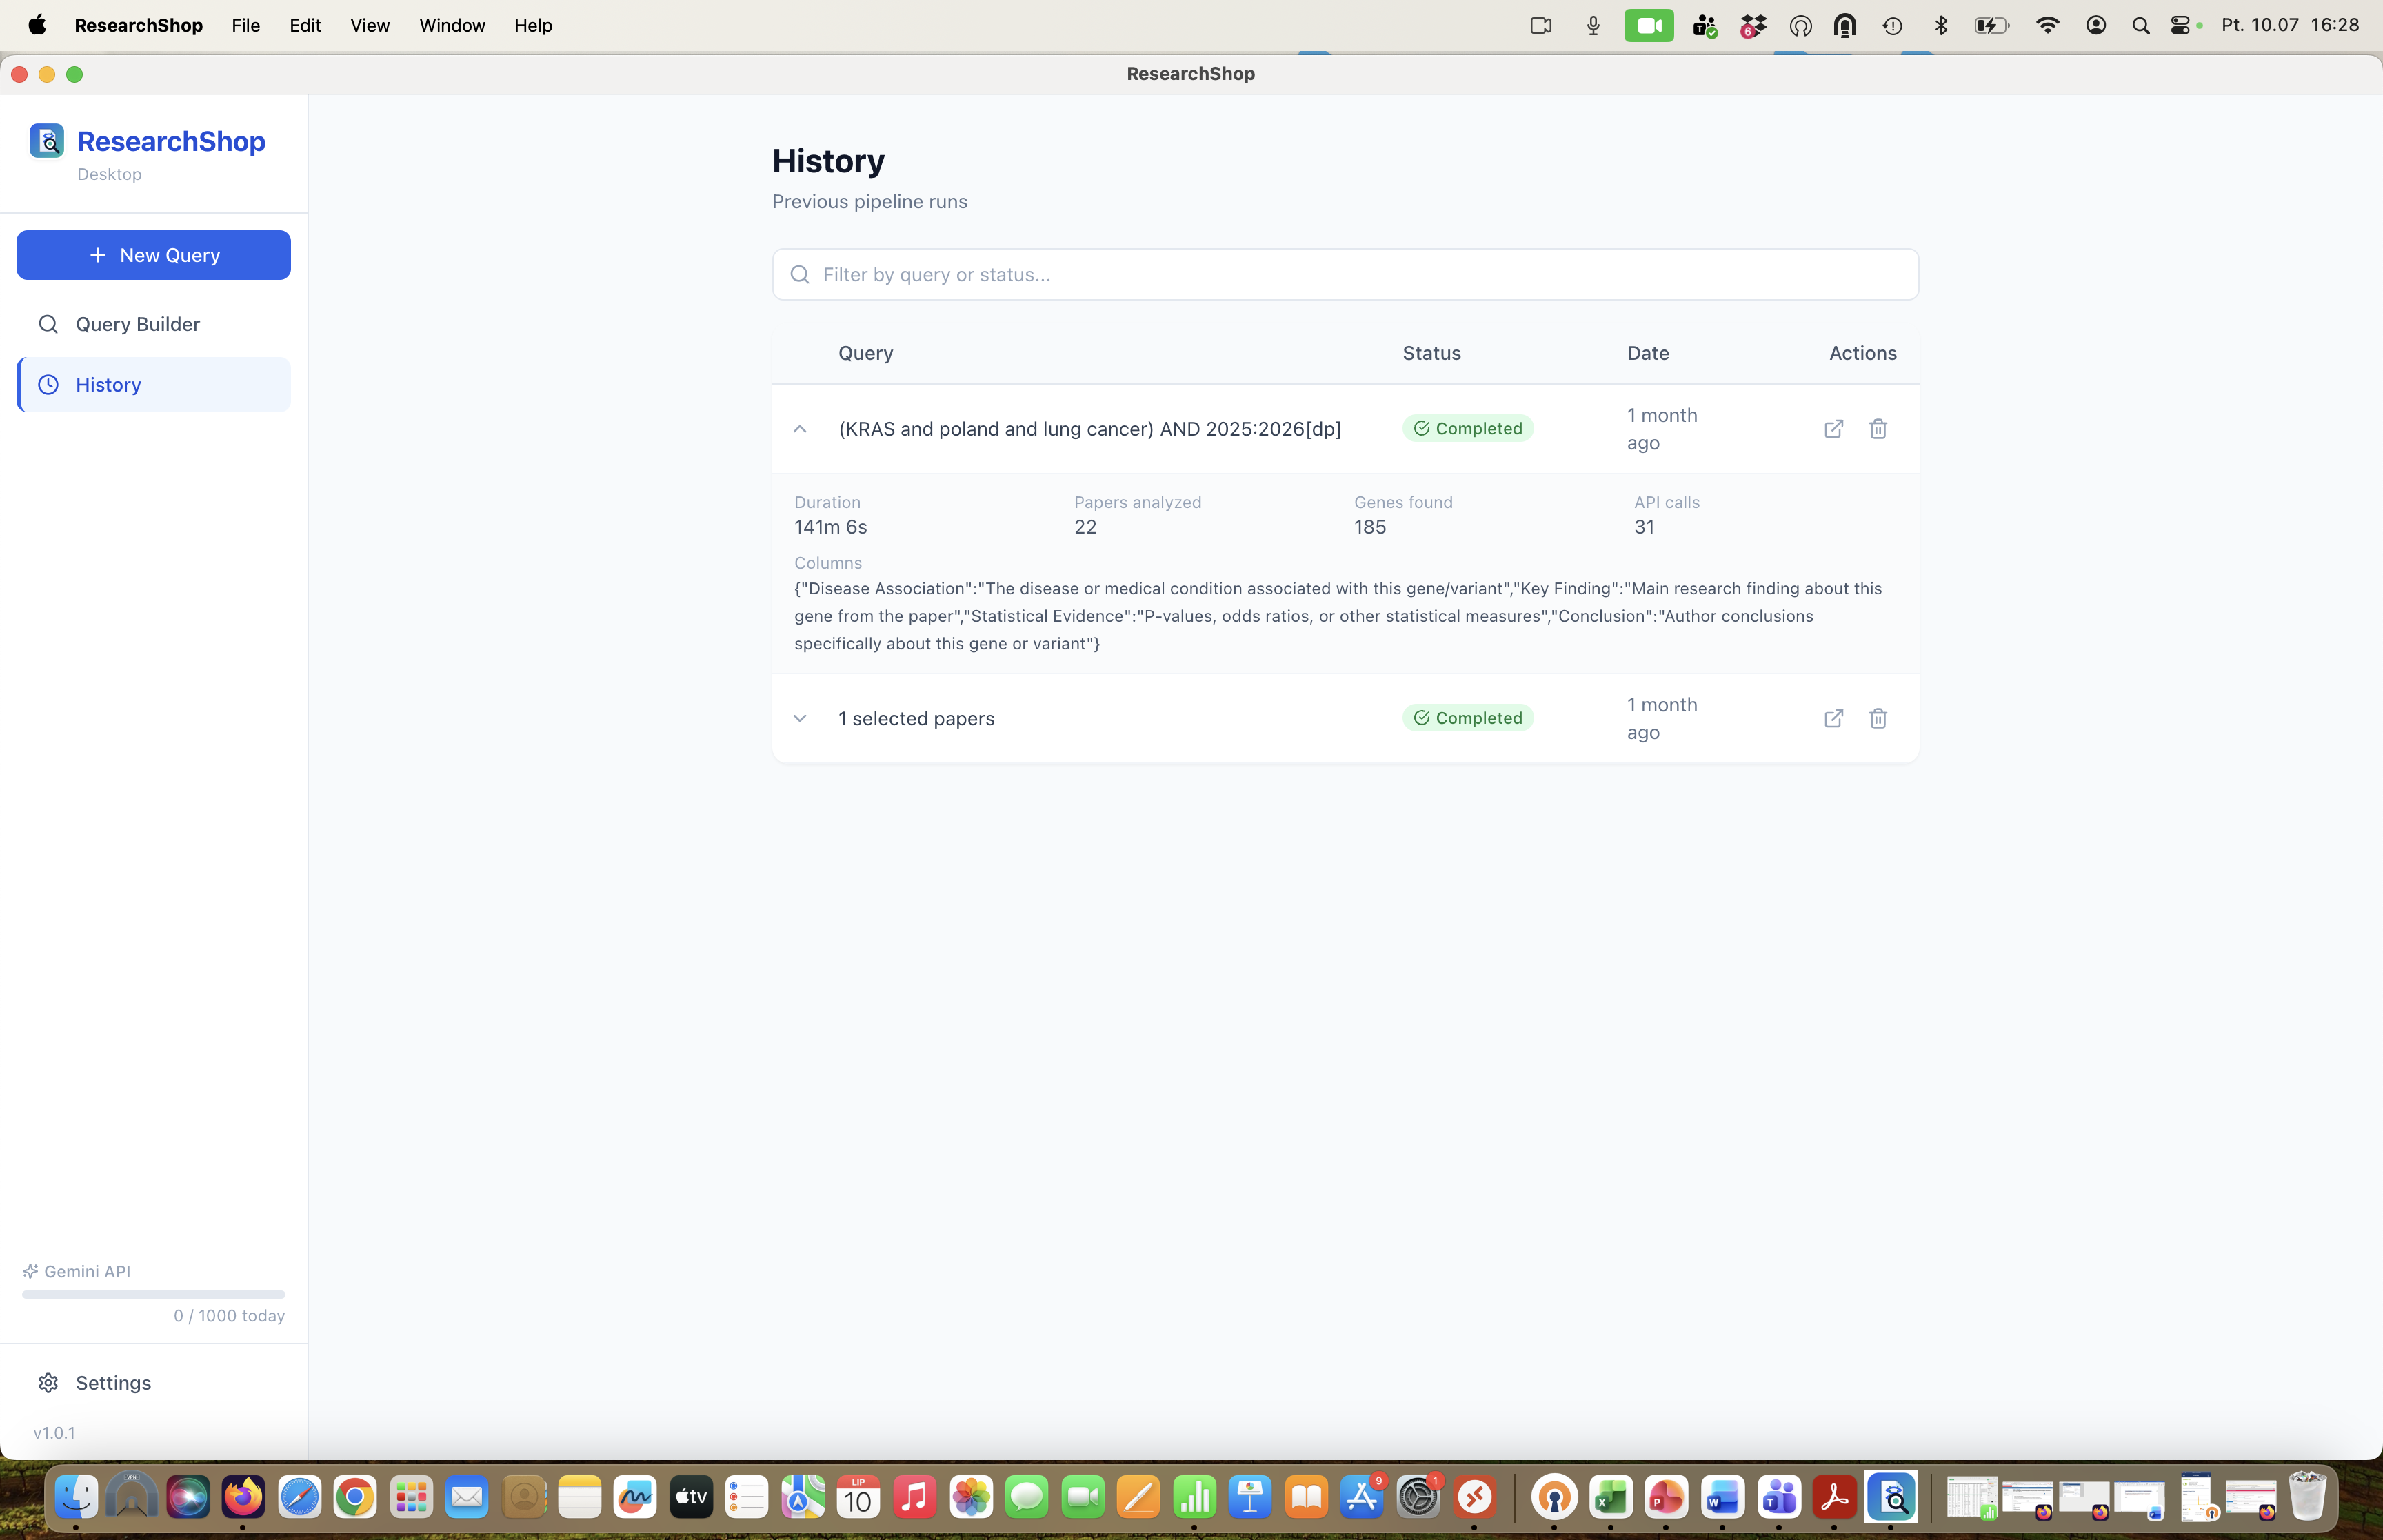
\includegraphics[width=0.96\textwidth,trim=525 540 250 90,clip]{figures/kras_example_history.png}
\par
\scriptsize (a) History: recorded query, duration, papers analysed, gene count, and API calls.
\par\medskip
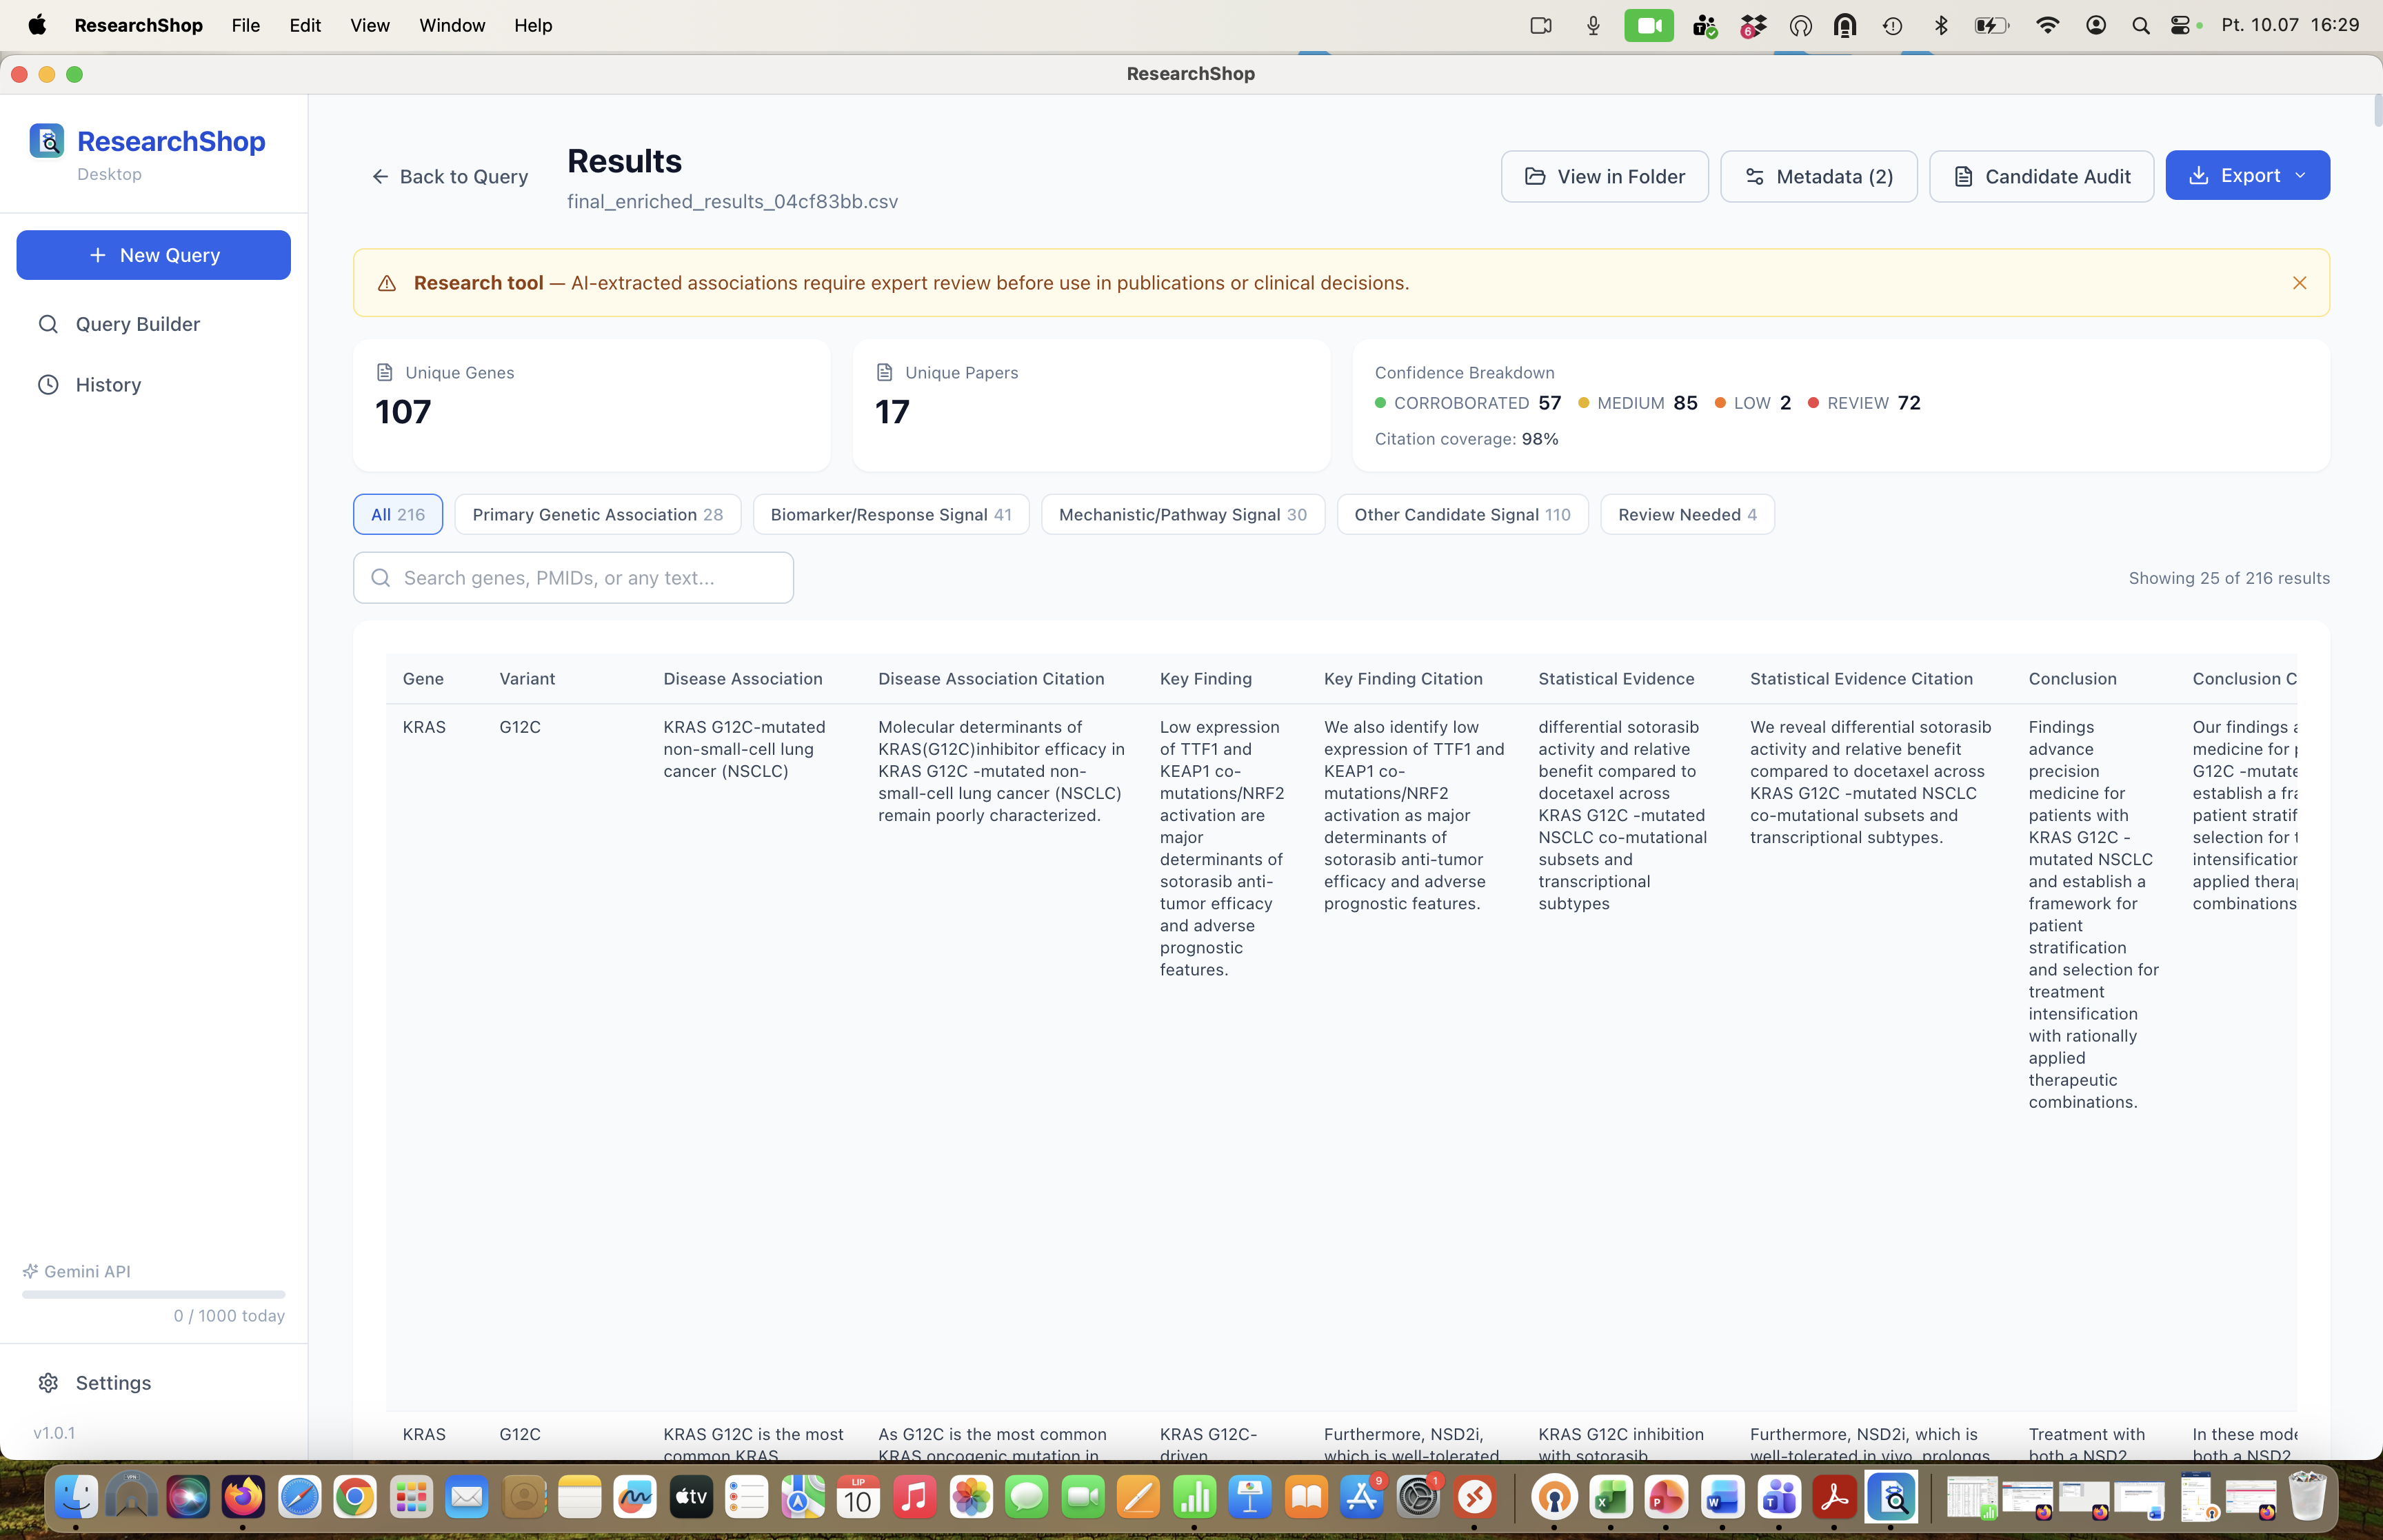
\includegraphics[width=0.96\textwidth,trim=260 320 35 85,clip]{figures/kras_example_results.png}
\par
\scriptsize (b) Results: final counts, confidence breakdown, and an exported KRAS row with source-citation fields.
\captionof{figure}{Recorded ResearchShop run for the KRAS query. Both panels use the same scale and aspect ratio so that the displayed values and output fields remain legible.}
\label{fig:app_workflow_screens}

\endgroup
\vspace{-0.6em}
\end{figure*}

\FloatBarrier
\subsection{Expert Assessment of Research Usefulness}
\label{sec:kras-expert-assessment}

\DIFaddbegin
\DIFadd{The operational checks above establish whether output can be traced to source text and whether the extraction workflow completes consistently. They do not determine whether a reported association is scientifically important or provides a useful research lead. That judgement requires review by a domain expert.}
\DIFaddend

\KasiaNote{Please select three to five representative findings from the supplied KRAS workbook, inspect their cited source passages, classify each finding as useful, not useful, or uncertain, and provide a short justification suitable for the final manuscript. No entry below has been selected or classified by the software or by AI.}

\begin{table}[H]
\centering
\caption{\DIFadd{Expert assessment template for the KRAS application example. This table is intentionally incomplete in the editorial draft and must not be interpreted as an accuracy result.}}
\label{tab:kras-expert-assessment}
\footnotesize
\setlength{\tabcolsep}{3pt}
\renewcommand{\arraystretch}{1.04}
\begin{tabularx}{\columnwidth}{@{}>{\raggedright\arraybackslash}p{0.45\columnwidth} >{\raggedright\arraybackslash}X@{}}
\toprule
\DIFadd{\textbf{Assessment item}} & \DIFadd{\textbf{Expert response}} \\
\midrule
\DIFadd{Representative KRAS findings selected for assessment} &
\rule{0pt}{2.2em}\DIFadd{\textit{Pending expert selection of 3--5 findings.}} \\
\DIFadd{Are the findings supported by the cited source passages?} &
\rule{0pt}{2.2em}\DIFadd{\textit{Pending expert assessment.}} \\
\DIFadd{Do the findings add useful information beyond the original query?} &
\rule{0pt}{2.2em}\DIFadd{\textit{Pending expert assessment.}} \\
\DIFadd{Which findings constitute useful research leads, and why?} &
\rule{0pt}{2.6em}\DIFadd{\textit{Pending expert assessment.}} \\
\DIFadd{Which findings are uninformative, misleading, or require exclusion?} &
\rule{0pt}{2.6em}\DIFadd{\textit{Pending expert assessment.}} \\
\DIFadd{Overall usefulness and suggested manuscript interpretation} &
\rule{0pt}{2.8em}\DIFadd{\textit{Pending expert conclusion.}} \\
\bottomrule
\end{tabularx}
\end{table}
